\documentclass[xcolor=dvipsnames]{beamer}
\usepackage{graphicx}
\usepackage{listings}
\usetheme{AnnArbor}
\usecolortheme{beaver}
\usepackage[utf8]{inputenc}
\usepackage[T1]{fontenc}
\usepackage[frenchb]{babel}
\usepackage{setspace}
\usepackage{color}
\graphicspath{ {pics/} }
%\usecolortheme[named=BurntOrange]
\title[]{Introduction a Akka}
\subtitle[]{Reactive  Programming \& Acteurs}
\author[]{J.MOLIERE-jerome@javaxpert.com}
\institute[]{Zenika}
\date{20140925}

\lstdefinelanguage{Scala}%
  {morekeywords={abstract,case,catch,class,def,%
    do,else,extends,false,final,finally,%
    for,if,implicit,import,lazy,match,mixin,%
    new,null,object,override,package,%
    private,protected,requires,return,sealed,%
    super,this,trait,true,try,%
    type,val,var,while,with,yield},%+
%       otherkeywords={_,:,=,=>,<<:,<\%,>:,\#,@},%
        otherkeywords={=,=>,<-,<\%,<:,>:,\#,@},%
   sensitive,%
   morecomment=[l]//,%
   morecomment=[n]{/*}{*/},%
   morestring=[b]",%
   morestring=[b]',%
   morestring=[b]""",%
  }[keywords,comments,strings]%

\begin{document}

\lstset{language=Scala}
\begin{frame}
\titlepage
\end{frame}
\section{Introduction}
\begin{frame}
  \frametitle{Ce jeu de slides}
  A propos de ces slides:
  \begin{itemize}
  \item produits avec \LaTeX sous Emacs
  \item geres en version sous Git
  \item tout cela sous Debian...
  \item version de Scala :2.11
  \item version de JVM utilisee : 1.8.020
  \end{itemize}
\end{frame}

\begin{frame}
  \frametitle{Acteurs}
   Les acteurs sont un des avatars du \textbf{Reactive Programming}.
   Un ensemble de \textbf{patterns} visant a construire des applications:
   \begin{itemize}
   \item tolerantes aux pannes,
   \item pouvant monter en charge,
   \item legeres en terme de ressources,
   \item multi threads sans gestion explicite de la concurrence.
   \end{itemize}
\end{frame}

\begin{frame}
  \frametitle{Les origines}
  Initialement integre dans le langage, un module de gestion des acteurs.Ce module a grossi , deborde le stade du simple module pour devenir un produit a part entiere :
  \begin{exampleblock}{}
  \begin{itemize}
   \item support officiel par TypeSafe,
   \item outillage d'administration/supervision,
   \item nombreux algorithmes de \textbf{load balancing},
   \item l'ancien framework integre au langage est dorenavant deprecie depuis la version 2.10.
  \end{itemize}
  \end{exampleblock}
\end{frame}

\begin{frame}
  \frametitle{But du framework Akka}
  Le framework Akka propose une solution couvrant l'ensemble des besoins pour une application critique:
  \begin{enumerate}
   \item distribution sur plusieurs machines
   \item  tolerance aux pannes
   \item supervision
   \item repartition de la charge
  \end{enumerate}
\end{frame}

\section{Concepts}
\begin{frame}
  \frametitle{Acteurs : definition}
  \begin{definition}
    Un acteur est une unite de calcul encapsulant:
    \begin{itemize}
   \item stockage
   \item traitement
   \item  communication
    \end{itemize}
  \end{definition}
\end{frame}

\begin{frame}[fragile]
  \frametitle{Entites en presence}
  \begin{figure}[h!]
  \caption{Acteurs \& entites}
  \centering
      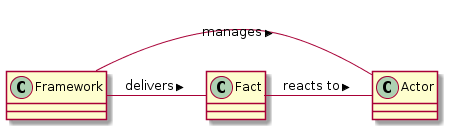
\includegraphics{akka-entities}
  \end{figure}
\end{frame}

\begin{frame}[fragile]
  \frametitle{Cycle de developpement classique}
   \begin{figure}[h!]
  \caption{Comment penser son application?}
  \centering
      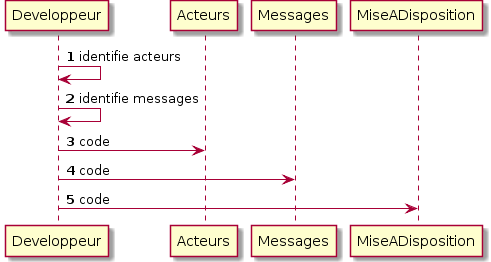
\includegraphics[scale=0.5]{akka-dev-cycle}
  \end{figure}
\end{frame}

\begin{frame}
  \frametitle{Acteurs et modelisation}
  Un acteur est une classe tres simple , reagissant a des evenements. Il convient de suivre quelques regles:
  \begin{itemize}
   \item heritage suivant le framework employe,
   \item redefinir les methodes idoines,
   \item  tenter de conserver les acteurs \textit{stateless},
   \item  tenter de faire en sorte qu'ils soient les plus simples possibles.
  \end{itemize}
\end{frame}
\subsection{Akka : le framework}
\begin{frame}[fragile]
  \frametitle{la classe Actor}
   \begin{figure}[h!]
  \caption{La classe Actor vue statique}
  \centering
      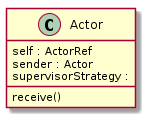
\includegraphics[scale=0.5]{akka-actor-class}
  \end{figure}
\end{frame}

\begin{frame}[fragile]
  \frametitle{Cycle de vie des acteurs}
    De nombreuses methodes se trouvent dans l'API permettant
   un controle total sur les transitions entre etats des acteurs.
   Methodes pre[StateName]\/post[StateName].
    \begin{figure}[h!]
  \caption{Cycle de vie}
  \centering
      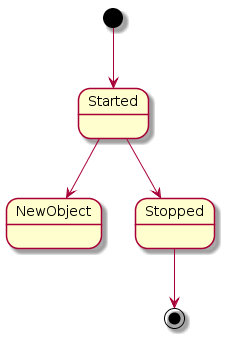
\includegraphics[scale=0.5]{akka-lifecycle.png}
  \end{figure}
\end{frame}

\begin{frame}[fragile]
  \frametitle{Cycle de vie des acteurs..Suite}
  Diagramme officiel extrait des documentations Akka officielles.
    \begin{figure}[h!]
  \caption{Cycle de vie}
  \centering
      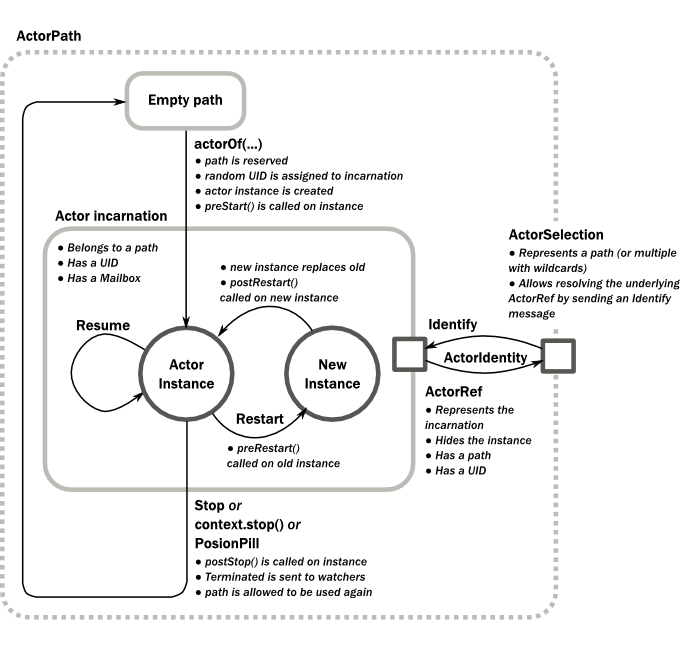
\includegraphics[scale=0.5]{actor_lifecycle1.png}
  \end{figure}
\end{frame}


\subsection{Communication asynchrone}
\begin{frame}
  \frametitle{Acteurs et communication}
  Les acteurs adoptent d'office un mode de communication asynchrone:
  \begin{enumerate}
  \item jamais de blocage du systeme,
  \item ideal en terme de montee en charge, deployer plus d'acteurs sur plus de machines induit une augmentation du throughput,
  \item plus simple a gerer pour la supervision, les \textit{timeouts} sont vite assimiles a des defauts applicatifss.
  \end{enumerate}
\end{frame}

\section{Developper avec Akka}
\subsection{Akka, vue logicielle}
\begin{frame}
  \frametitle{Akka \& Composants}
  Akka est un ensemble de composants parmi lesquels:
  \begin{enumerate}
  \item une API
  \item une console de supervision
  \item un DSL
  \end{enumerate}
  La partie client-serveur utilise Netty, le projet JBoss de
  serveur TCP NIO.
\end{frame}

\subsection{Quick start Akka}
\begin{frame}
  \frametitle{Droit au code}
  Apres cette introduction generale, regardons la mise en place d'unacteur avec Akka:
  \begin{enumerate}
   \item codage d'un acteur,
   \item codage d'un message,
   \item classe principale (manipulation du framework),
   \item definition generale du projet SBT,
   \item  mise en place sur une machine.
  \end{enumerate}
  Rien de tel qu'un bon vieux Hello World...
\end{frame}

\begin{frame}[fragile]
  \frametitle{Un acteur basique}
  \lstset{frameround=fttt}
\begin{lstlisting}[frame=trBL]
import akka.actor.Actor
import akka.actor.ActorSystem
import akka.actor.Props
class HelloActor extends Actor {
  def receive = {
    case "hello" => println("hello")
    case _       => println("Sorry!!")
  }
}
  \end{lstlisting}
\end{frame}

\begin{frame}[fragile]
  \frametitle{Mise a disposition de l'acteur}
   \lstset{frameround=fttt}
\begin{lstlisting}[frame=trBL]
  object Main extends App {
  val system = ActorSystem("HelloSystem")
  // default Actor constructor
  val helloActor = system.actorOf(
  Props[HelloActor], name = "helloactor")
  helloActor ! "hello"
  helloActor ! "buenos dias"
  }
\end{lstlisting}
\end{frame}

\begin{frame}[fragile]
  \frametitle{Script SBT du projet}
  %% \begin{verbatim}
    \lstset{frameround=fttt}
\begin{lstlisting}[frame=trBL]
name := "Actor basic #1"

version := "1.0"

scalaVersion := "2.11.0"

resolvers += "Typesafe Repository" \
at "http://repo.typesafe.com/typesafe/releases/"

libraryDependencies += "com.typesafe.akka" % "akka-actor_2.11"\
% "2.3.6"
\end{lstlisting}
%%\end{verbatim}
\end{frame}

\begin{frame}
  \frametitle{Ce qu'il faut retenir...}
  Points essentiels mis en evidence par l'exemple:
  \begin{enumerate}
  \item heriter du trait \textit{Actor},
  \item redefinir la methode \textit{receive}, indiquant la reaction adaptee a chaque type de message,
  \item envoi de messages entre acteurs via !
  \end{enumerate}
\end{frame}

\subsection{Exemple avance}
\begin{frame}
  \frametitle{Introduction}
  Nous allons mettre en place un ping-pong avec Akka.
  Les entites en lice sont:
  \begin{itemize}
  \item un acteur \textbf{Ping} reagissant aux messages \textbf{Pong} et \textbf{Halt}
  \item un acteur \textbf{Pong} reagissant aux messages \textbf{Ping} et \textbf{Init}
  \item une classe mettant a disposition les objets et initialisant le dialogue
  \end{itemize}
  Au bout de \textit{n} echanges le dialogue est rompu.
\end{frame}

\begin{frame}[fragile]
  \frametitle{Modelisation}
   \begin{figure}[h!]
  \caption{Acteurs \& entites}
  \centering
      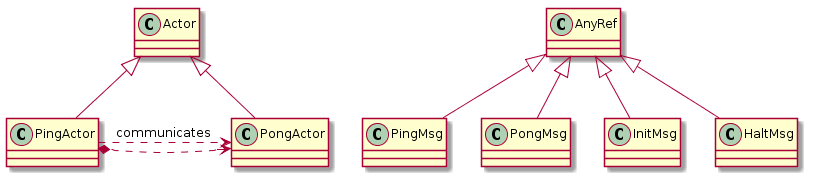
\includegraphics[scale=0.25]{pingpong-classes}
   \end{figure}
\end{frame}

\begin{frame}[fragile]
  \frametitle{Dialogue}
  \begin{figure}[h!]
  \caption{Dialogue entre acteurs}
  \centering
      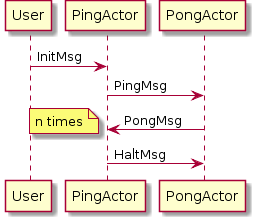
\includegraphics[scale=0.5]{pingpong-sequence}
   \end{figure}
\end{frame}

\begin{frame}[fragile]
  \frametitle{Les messages}
    \lstset{frameround=fttt}
    \begin{lstlisting}[frame=trBL]
package pingpong.msg
case object InitMsg
case object PongMsg
case object HaltMsg
case object PingMsg
    \end{lstlisting}
\end{frame}

\begin{frame}[fragile]
  \frametitle{Acteur Pong}
  \lstset{frameround=fttt}
  \begin{lstlisting}[frame=trBL]
package pingpong.actors
import akka.actor.*
import pingpong.msg.*
class PongActor extends Actor {
  var counter = 0
  def newPing (sender : ActorRef) = {
    counter+=1
    println("received a new Ping")
    if(counter<3)
      sender ! PongMsg
    else{
      println("Max value reached ..!")
      sender ! HaltMsg} }
  \end{lstlisting}
\end{frame}


\begin{frame}[fragile]
  \frametitle{Acteur Pong..suite}
  \lstset{frameround=fttt}
  \begin{lstlisting}[frame=trBL]
  def receive = {
    case PingMsg =>
      newPing(sender)
    case _ => println("oops!!!")
  }
}
  \end{lstlisting}
\end{frame}


\begin{frame}[fragile]
  \frametitle{Acteur Ping..}
  \lstset{frameround=fttt}
  \begin{lstlisting}[frame=trBL]
class PingActor(pong : ActorRef) extends Actor {
  var started = false
  def receive = {
    case InitMsg =>
      started = true
      println( "Ok starting with a Ping to Pong")
      pong ! PingMsg
    case PongMsg =>
      println("received Pong messag")
      if(!started)
        println("Discarded not yet started!!")
      else{
        sender ! PingMsg
        println ( "replying to Pong with Ping")}
  \end{lstlisting}
\end{frame}

\begin{frame}[fragile]
 \lstset{frameround=fttt}
  \begin{lstlisting}[frame=trBL]
    case HaltMsg =>
        started = false
        println ( "HaltMsg received")
        //context.stop(self)
        case _ => println( )}}
  \end{lstlisting}
\end{frame}

\begin{frame}[fragile]
  \frametitle{Programme principal}
 \lstset{frameround=fttt}
  \begin{lstlisting}[frame=trBL]
// imports omis
object Main extends App {
  println("Starting PingPong")
  val system = ActorSystem("PingPongSystem")
  val pong = system.actorOf(Props[PongActor]
  , name = "pong")
  val ping = system.actorOf(Props
  (new PingActor(pong)), name = "ping")
  println("Sending InitMsg")
  ping ! InitMsg
}
\end{lstlisting}
\end{frame}

\begin{frame}[fragile]
  \frametitle{Execution du programme}
  \begin{lstlisting}[frame=trBL]
Starting PingPong
Got the actors references ...Sending InitMsg
Ok starting with a Ping to Pong
received a new Ping
received Pong messag
received a new Ping
replying to Pong with Ping
received Pong messag
replying to Pong with Ping
received a new Ping
Max value reached ..!!!Leaving...
HaltMsg received - toggled flag
\end{lstlisting}
\end{frame}

 \begin{frame}
   \frametitle{Ce qu'il faut retenir}
   Points a souligner :
   \begin{itemize}
   \item les messages sont simplistes et ne contiennent pas d'information d'ou utilisation de \textbf{case object},
   \item  possibilite de stopper le programme en supprimant la reference d'acteur via \textit{context.stop(self)},
   \item la reference sur l'objet courant self,
   \item le fonctionnement proche de RMI \/JNDI (\textbf{annuaire}),
   \end{itemize}
 \end{frame}

\section{Akka avance}
\subsection{Configuration}
\begin{frame}
  \frametitle{Introduction}
  Akka est \textit{extremement configurable}:
  \begin{itemize}
  \item utilise TypeSafe Config le framework de TypeSafe:
    \begin{itemize}
    \item syntaxe proche de JSON et de l'EDN Clojure
    \item donc proche de JSON
    \item couples cles \& valeurs hierarchisees
    \end{itemize}
  \item permet de specifier de nombreux parametres:
    \begin{itemize}
    \item pooling (ExecutorService)
    \item routage
    \item specification du typage des messages achemines sur les acteurs
    \item deploiement
    \item supervision
    \end{itemize}
  \end{itemize}
\end{frame}

  \begin{frame}
    \frametitle{Configurer : dans quels cas?}
    Pour des besoins avances ou pour tester des cas specifiques:
    \begin{itemize}
    \item developpement sur plusieurs noeuds,
    \item diverses instances sur la meme machine (developpement \& recette),
    \item pour ameliorer la robustesse de votre solution.
    \end{itemize}
    Par defaut, nul besoin de configuration explicite.
  \end{frame}

  \begin{frame}[fragile]
    \frametitle{Configuration exemple}
    \begin{lstlisting}[frame=trBL]
akka {
  loggers = ["akka.event.slf4j.Slf4jLogger"]
  loglevel = "DEBUG"
  actor {
    provider = "akka.cluster.ClusterActorRefProvider"
    default-dispatcher {
      throughput = 10
    }
  }
  remote {
    netty.tcp.port = 4711
  }
}
\end{lstlisting}
\end{frame}

\subsection{la console Akka}
\begin{frame}
  \frametitle{Introduction}
  La console Akka permet de superviser son application et de monitorer le fonctionnement de celle-ci en:
  \begin{itemize}
  \item echantillonant les reactions de l'application dans le cas d'envoi de messages,
  \item stockant les resultats de cet echantillonnage dans une base de donnees,
  \item en offrant une restitution visuelle.
  \end{itemize}
\end{frame}

\begin{frame}
  \frametitle{Concepts}
  L'echantillonnage realise par la console n'est que du code insere
  directement dans votre \textbf{bytecode} par un framework d'\textbf{AOP}.
  \begin{alertblock}{Consequence}
  Il faudra donc activer et configurer explicitement les acteurs
  concernes par ces mesures et la frequence de celle-ci.
\end{alertblock}
\end{frame}

\begin{frame}[fragile]
  \frametitle{Configuration sur une application}
  Il faudra rajouter dans votre \textit{application.conf} un bloc du type.
  \begin{lstlisting}[frame=trBL]
      atmos {
      trace {
        enabled = true
        event-handlers =
        ["akka.atmos.trace.store.mongo.
        MongoTraceEventListener"]
        mongo {
          db-name = "atmos-monitoring"
          db-connection-uri = "mongodb://localhost"
        }
      }
    }
  \end{lstlisting}
\end{frame}

\section{Conclusions}
\begin{frame}
  \frametitle{On aurait pu parler de}
  Voila pour cet examen detaille du framework qui n'aborde pas
  tout l'ensemble des possibilites offertes par Akka car on aurait
  pu aussi:
  \begin{itemize}
  \item parler de la personnalisation du framework avec les possibilites d'implementations de divers traits offerts par le framework,
  \item se pencher plus sur la personnalisation,
  \item entrer dans la mecanique de reprise sur erreur,
  \item aborder la performance, l'audit ...
  \item etc...
  \end{itemize}
\end{frame}

\begin{frame}
  \frametitle{Questions \& Commentaires}
  Remarques bienvenues...
  Des questions ?
\end{frame}

\section{Labs}
\begin{frame}
  \frametitle{Skype en Scala - Partie 1}
  Le sujet de ce TP est de construire les briques d'un moteur de messagerie instantanee.
  Pour cela il sera bon de :
  \begin{itemize}
  \item lister les acteurs en lice,
  \item lister les messages echanges,
  \item bref suivre la methode vue dans cette section.
  \end{itemize}
  Implementer et tester cette premiere partie dans la VM.
\end{frame}

\begin{frame}
  \frametitle{Skype en Scala - Partie 2}
  Ici nous allons passer a un deploiement en reseau des acteurs.
  Pour tester cette partie il faudra modifier la configuration de
  la VM:
  \begin{enumerate}
  \item stopper la VM
  \item cliquer bouton droit dans VirtualBox
  \item aller dans preferences/settings
  \item selectionner le menu reseau
  \item ajouter une seconde carte reseau (une par defaut em mode NAT)
  \end{enumerate}
  Si la configuration de la salle le permet on devrait pouvoir communiquer entre VMs dans la salle via une configuration en mode \textbf{bridge}. Si celle-ci ne fonctionne pas et que les machines sont assez puissantes on peut tenter de  lancer 2 VMs sur la meme machine hote en mode \textbf{reseau prive}.
\end{frame}

\begin{frame}
  \frametitle{Skype en Scala - Partie 3}
  Pour ceux motives pour arriver ici, nous allons ajouter ici:
  \begin{itemize}
  \item supervision avec la console Akka,
  \item tests de diverses strategies,
  \end{itemize}
\end{frame}

\section{Annexes}
\subsection{Utilisation de la machine virtuelle}
\begin{frame}
  \frametitle{Demarrage}
  \begin{enumerate}
  \item lancer VirtualBox
  \item importer la VM (.ova)
  \item une fois le processus termine, cliquer sur la VM apparue dans la liste et cliquer sur start,
  \item apres quelques secondes, un ecran de connexion apparait
  \item utiliser \textbf{user} et {testp} pour vous connecter
  \end{enumerate}
\end{frame}

\begin{frame}[fragile]
  \frametitle{Travailler avec la VM}
  Il s'agit d'un Linux base sur du Debian stable (wheezy).
  L'ensemble des documents, des exemples et des binaires lies a Scala
  sont rassembles dans le dossier \textbf{platform} dans le compte utilisateur.
\begin{verbatim}
cd ~
cd platform
ls -la
\end{verbatim}
\end{frame}

\begin{frame}[fragile]
  \frametitle{Installer des paquets}
  Si certains logiciels manquent a l'appel vous pouvez en installer:
  \begin{itemize}
  \item dans un terminal par \textbf{apt-get} ou \textbf{aptitude}
  \item graphiquement par \textbf{synaptic} disponible dans les menus (bouton droit sur le bureau)
  \end{itemize}
\begin{verbatim}
>aptitude search scala
>sudo aptitude install scala
\end{verbatim}
\end{frame}

\end{document}
